\documentclass[a4paper,12pt,oneside]{report}
\usepackage{graphicx}
\usepackage{color}
\usepackage{url}
\usepackage{subfigure}
\usepackage[utf8]{inputenc}
\usepackage[T1]{fontenc}
\usepackage{tgpagella}
\usepackage{xstring}
\usepackage{wrapfig}
\usepackage{appendix}
\usepackage{nomencl}
\usepackage{algorithm}
\usepackage{algorithmic}
\usepackage{multicol}
\usepackage[pdfborder=0 0 0]{hyperref}
\usepackage{amssymb}
\usepackage{amsthm}

\newcommand{\myscale}{0.74}
\newcommand{\vect}[1]{\boldsymbol{#1}}
\newcommand{\code}[1]{\texttt{\StrSubstitute{#1}{.}{.\.}}}
\def\.{\discretionary{}{}{}}
\newcommand{\heu}[1]{\texttt{\textit{#1}}}
\newcommand{\jmodule}[1]{\texttt{\textit{#1}}}
\linespread{1.5}

\renewcommand{\algorithmicrequire}{\textbf{Input:}}
\renewcommand{\algorithmicensure}{\textbf{Output:}}
\renewcommand{\algorithmicforall}{\textbf{for each}}
\renewcommand{\algorithmiccomment}[1]{\textit{// #1}}

\renewcommand{\nomname}{List of Abbreviations}
\makenomenclature

\theoremstyle{definition}
\newtheorem{define}{Definition}[chapter]

\setlength{\hoffset}{-1in} %left margin will be 0, as hoffset is by default 1inch
\setlength{\voffset}{-1in} %analogous voffset
\setlength{\oddsidemargin}{4cm}
\setlength{\evensidemargin}{4cm}
\setlength{\topmargin}{25mm}
\setlength{\footskip}{1cm}
\setlength{\headheight}{0cm}
\setlength{\headsep}{0cm}
\setlength{\marginparwidth}{0cm}
\setlength{\marginparpush}{0cm}
\setlength{\textheight}{23.7cm}
\setlength{\textwidth}{14.5cm}
\let\openright=\clearpage

\def\mfauthor{Matej Vitásek}
\def\mfadvisor{RNDr. Irena Mlýnková Ph.D.}
\def\mfplacedate{Praha, 2011}

% Tato makra přesvědčují mírně ošklivým trikem LaTeX, aby hlavičky kapitol
% sázel příčetněji a nevynechával nad nimi spoustu místa. Směle ignorujte.
\makeatletter
\def\@makechapterhead#1{
  {\parindent \z@ \raggedright \normalfont
   \Huge\bfseries \thechapter. #1
   \par\nobreak
   \vskip 20\p@
}}
\def\@makeschapterhead#1{
  {\parindent \z@ \raggedright \normalfont
   \Huge\bfseries #1
   \par\nobreak
   \vskip 20\p@
}}
\makeatother

\def\chapwithtoc#1{
\chapter*{#1}
\addcontentsline{toc}{chapter}{#1}
}

\begin{document}

\lefthyphenmin=2
\righthyphenmin=2

%%% Titulní strana práce ======================================================
\pagestyle{empty}
\begin{center}

\large

Charles University in Prague

\medskip

Faculty of Mathematics and Physics

\vfill

{\bf\Large MASTER THESIS}

\vfill

\centerline{\mbox{
\includegraphics[width=60mm]{logo}}}

\vfill
\vspace{5mm}

{\LARGE \mfauthor}

\vspace{15mm}

% exactly as assigned
{\LARGE\bfseries Inference of XML Integrity Constraints}

\vfill

% Název katedry nebo ústavu, kde byla práce oficiálně zadána
% (dle Organizační struktury MFF UK)
Department of Software Engineering

\vfill

\begin{tabular}{rl}

Supervisor of the master thesis: & 	\mfadvisor \\
\noalign{\vspace{2mm}}
Study programme: & Informatika \\
\noalign{\vspace{2mm}}
Specialization: & ISS \\
\end{tabular}

\vfill

% Zde doplňte rok
\mfplacedate 

\end{center}



\newpage % ============================================================
%%% Následuje vevázaný list -- kopie podepsaného "Zadání diplomové práce".
%%% Toto zadání NENÍ součástí elektronické verze práce, nescanovat.
\openright

\noindent
[Sample: Here you may thank whoever you wish (the supervisor of the thesis, the consultant,
the person who lent the software, literature, etc.)]

TODO thank jInfer team, Mlynkova, anyone helping create this, colleagues at work...


\newpage % ============================================================
%%% Strana s čestným prohlášením k diplomové práci
\vglue 0pt plus 1fill
\noindent
I declare that I carried out this master thesis independently, and only with the cited
sources, literature and other professional sources.

\medskip\noindent
I understand that my work relates to the rights and obligations under the Act No.
121/2000 Coll., the Copyright Act, as amended, in particular the fact that the Charles
University in Prague has the right to conclude a license agreement on the use of this
work as a school work pursuant to Section 60 paragraph 1 of the Copyright Act.

\vspace{10mm}

\hbox{\hbox to 0.5\hsize{%
In ........ date ............
\hss}\hbox to 0.5\hsize{%
signature
\hss}}

\vspace{20mm}



\newpage % ============================================================
%%% Povinná informační strana diplomové práce
\vbox to 0.5\vsize{
\setlength\parindent{0mm}
\setlength\parskip{5mm}

Název práce: Odvozování integritních omezení v XML % TODO how to translate this correctly?

Autor: \mfauthor

Katedra:  Katedra softwarového inženýrství

Vedoucí diplomové práce: \mfadvisor{}, Katedra softwarového inženýrství

Abstrakt: [abstract of 80-200 words in Czech, but not a copy of the assignment of the
master thesis]

Klíčová slova:  XML, ID atributy, odvozování

\vss}\nobreak\vbox to 0.49\vsize{
\setlength\parindent{0mm}
\setlength\parskip{5mm}

Title:  Inference of XML Integrity Constraints

Author: \mfauthor

Department: Department of Software Engineering

Supervisor: \mfadvisor{}, Department of Software Engineering

Abstract:  [abstract of 80-200 words in English, but not a copy of the assignment of
the master thesis]

Keywords: XML, ID attributes, inference

\vss}

\newpage

%%% Strana s automaticky generovaným obsahem diplomové práce. U matematických
%%% prací je přípustné, aby seznam tabulek a zkratek, existují-li, byl umístěn
%%% na začátku práce, místo na jejím konci.

\openright
\pagestyle{plain}
\setcounter{page}{1}
\tableofcontents

% =============== TEXT ================
\newpage

% TODO what style of quotation marks to use? 
% TODO how to format text? is textit / texttt / ... OK?

\chapwithtoc{Preface}

Along with technologies like JSON, SQL/noSQL databases and bla, XML is one of the leading formats for storing structured data. However, even though languages such as DTD and XML Schema to describe XML structure already exist since a long time, most of the documents use outdated or no schema at all (link Vosta's Even ant can create...). To tackle this problem one may employ reverse-engineering techniques to infer the schema from existing documents, such as those described in A, B, C, jInfer. But the schema is not the only constraint that can be imposed on an XML document: the concept of \textit{keys} and \textit{foreign keys}, well known from the relational database world, applies here as well. One could go even further and try to find even more sophisticated relations in the data, such as \textit{functional dependencies} (link Sviro).

This work will be building upon the achievements of jInfer schema inference framework (TODO link Anti's improvements in schema inference), expanding its possibilities in the field of search for \textit{key-} and \textit{foreign key-}like structures in existing XML documents.

TODO Integrity constraints can be keys (with ID attributes as a "sub-group"), FKs, functional dependencies (quote Sviro), etc.
We will focus on the first kind - ID and IDREF attributes.

TODO argument: test data with DTD (and thus possibly ID/IDREF) is more common, we can have better test sets.

\section{Structure of the thesis}

The thesis will be structured as follows. 

First, we will introduce a few notions required throughout the work, such as XML tree, ID attributes, ID sets and keys for XML. 

Secondly, we will review approaches to ID attribute and XML keys search from previous articles on this topic. 

This will lead us to the NP-complete problem of maximal independent set (IS)\nomenclature{IS}{Independent Set}, where we will inspect approaches for solving it.

We will discuss a closely related Mixed Integer Problem (MIP)\nomenclature{MIP}{Mixed Integer Problem} and prove their "equality".

Afterwards, we will show how to use an external MIP solver and various heuristics to tackle this problem.

An extension to jInfer for finding ID attributes using MIP solver and a combination of heuristics will be presented and experimentally evaluated in the closing chapters.

\section{Conventions}

TODO list conventions - how we write code related stuff, module names, heu names, etc

\chapter{Definitions}

\begin{itemize}
	\item XML tree - from FIDAX or wherever
	\item Element, Attribute
	\item ID, IDREF, IDREFS attribute according to specification
	\item XSD keys (compare them to ID attributes)
	\item Key according to Keys for XML \cite{keX}
	\item Attribute mapping \nomenclature{AM}{Attribute Mapping}
	\item ID set
  \item Weight: support, coverage
\end{itemize}

\chapter{Research}

According to the article \cite{fidax}, ...

TODO talk about FIDAX
To the best of our knowledge, there are no other articles dealing with this problem. 

TODO talk about Fajt - but that's different, that's keys
TODO add citation for Fajt

\section{Independent Set}

TODO define IS + MIS rigorously

TODO other approaches to max IS

\chapter{MIP Approach}

TODO rigorously define MIP - optimization problem, some of the variables integral

TODO FIDAX is cool, but their heuristic might not be the best. It is a IS problem, let's try a multi-purpose solver. Use GLPK. \nomenclature{GLPK}{GNU Linear Programming Kit}

\section{Finding ID sets with GLPK}

TODO how GLPK works (branch \& bound), how to construct a problem, how output looks, how to interpret it, limit time-> limit quality, ...
 
 -> wow, GLPK works. However, it takes too long to get to optimum (link experiments), so let's try other heuristics.
 
\section{Heuristics}

TODO what is heuristics (link wise books), what is metaheuristics (we will be using them)

TODO mention things like Taboo search and Genetic Algorithms (we can emulate them with Crossover/Mutation) (we won't be using them)

TODO we will be working with heuristics striving to do the following: input is a list of AMs, they have their weight, we try to find a non-conflicting subset which maximizes the weight

TODO we will be using a pool - what is a pool

\begin{figure}
  \caption{Metaheuristic schema}
  \label{image-metaheuristic}
  \centering
    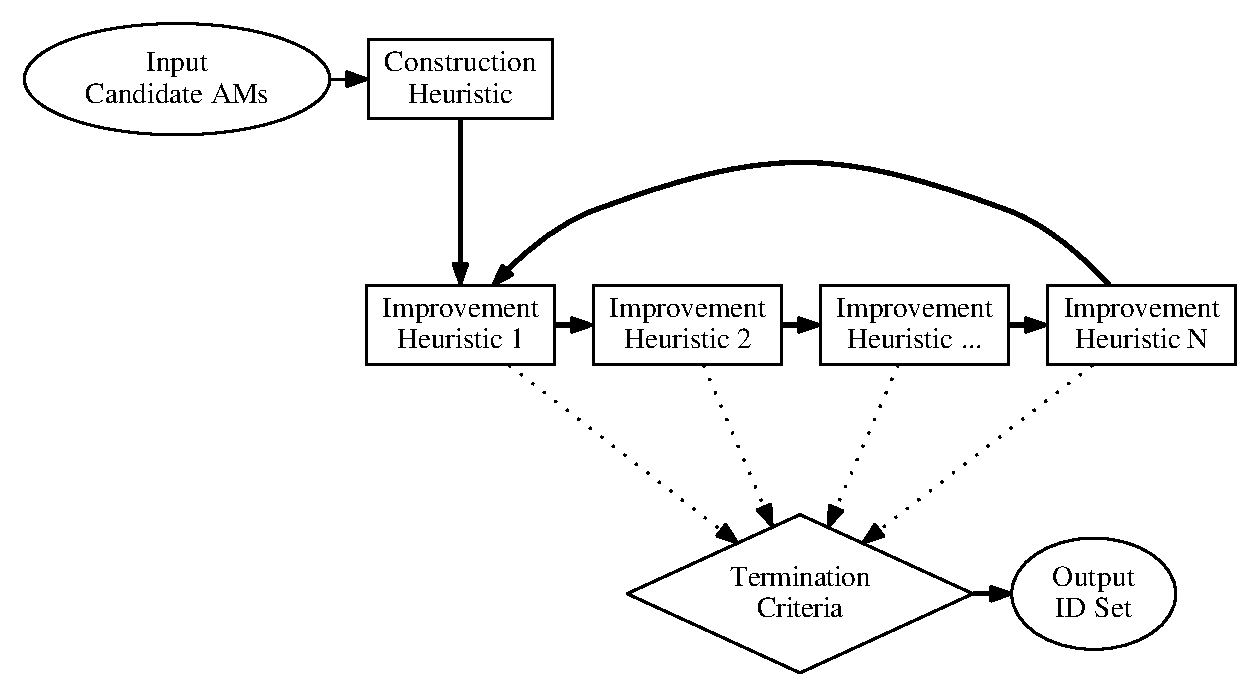
\includegraphics[width=\textwidth]{images/metaheuristic}
\end{figure}

\subsection{Constructions Heuristics}
% TODO can I format things in nomenclature?
\nomenclature{CH}{Construction Heuristic} %TODO decide on how to format CH/IH 

TODO construction heuristics are heus that provide us with at least some solution.

\subsubsection{FIDAX}

TODO this is a heuristic too! We can start with it!

The pseudocode is listed (cited from \cite{fidax} with trivial modifications without changing the logic) in \ref{ch-fidax}.

\begin{algorithm}
\caption{FIDAX CH}
\label{ch-fidax}
\begin{algorithmic}
\REQUIRE $C$ list of candidate AMs
\STATE $C' \gets C$ sorted by decreasing size
\STATE Compute the weight $w(m)$ of each $m$ in $C$
\FORALL{$t$ in $\Sigma^E$}
  \STATE Let $m$ be a \textbf{highest-weight} mapping of type $t$ in $C'$
  \STATE Remove from $C'$ all mappings of type $t$ except $m$
\ENDFOR
\FORALL{$m$ in $C'$}
  \STATE $S \gets$ all mappings in $C$ whose images intersect $\iota(m)$
  \IF{$w(m) > \sum_{p \in S} w(p)$}
    \STATE remove all $p \in S$ from $C'$
  \ELSE
    \STATE remove $m$ from $C'$
  \ENDIF
\ENDFOR
\RETURN $C'$
\end{algorithmic}
\end{algorithm}

\subsubsection{Random}

TODO this is trivial, but works - link experiments where it bashes FIDAX

See listing \ref{ch-random}.

\begin{algorithm}
\caption{Random CH}
\label{ch-random}
\begin{algorithmic}
\REQUIRE $N$ required size of pool
\REQUIRE $C$ list of candidate AMs
\ENSURE pool of $N$ feasible solutions
\STATE $r \gets $ empty pool
\FOR{$i = 1 \to N$} 
  \STATE \COMMENT{create 1 solution}
  \STATE $s \gets $ empty solution
  \WHILE{$s$ is a feasible ID set}
    \STATE $a \gets $ pick at random from $C \backslash S$
    \STATE $s \gets s \cup a$
  \ENDWHILE
  \STATE $r \gets r \cup s$
\ENDFOR
\RETURN $r$
\end{algorithmic}
\end{algorithm}

\subsubsection{Fuzzy}

TODO kind of trivial

See listing \ref{ch-fuzzy}.

\begin{algorithm}
\caption{Fuzzy CH}
\label{ch-fuzzy}
\begin{algorithmic}
\REQUIRE $N$ required size of pool
\REQUIRE $C$ list of candidate AMs
\ENSURE pool of $N$ feasible solutions
\STATE $r \gets $ empty pool
\FOR{$i = 1 \to N$} 
  \STATE \COMMENT{create 1 solution}
  \STATE $s \gets $ empty solution
  \STATE $C' \gets C$

  \WHILE{$C' $ not empty}
    \STATE $a \gets $ pick at weighted random from $C'$
    \IF{$s \cup a$ is a feasible ID set}
      \STATE $s \gets s \cup a$
      \STATE $C' \gets C' \backslash a$
    \ENDIF
    \FORALL{$c \in C'$}
      \IF{$s \cup c $ is \textbf{not} a feasible ID set}
        \STATE \COMMENT {if $c$ cannot be possibly added anymore}
        \STATE $C' \gets C' \backslash c$
      \ENDIF
    \ENDFOR
  \ENDWHILE

  \STATE $r \gets r + s$
\ENDFOR
\RETURN $r$
\end{algorithmic}
\end{algorithm}

\subsubsection{Incremental}

TODO trivial, hungry, always 1 solution

See listing \ref{ch-incremental}.

\begin{algorithm}
\caption{Incremental CH}
\label{ch-incremental}
\begin{algorithmic}
\REQUIRE $C$ list of candidate AMs
\ENSURE a feasible solution
\STATE $C' \gets $ sort $C$ by decreasing weight
\STATE $s \gets $ empty solution
\FORALL{$c \in C'$}
  \IF{$s \cup c$ is a feasible ID set}
    \STATE $s \gets s + c$
  \ENDIF
\ENDFOR
\RETURN $s$
\end{algorithmic}
\end{algorithm}

\subsubsection{Removal}

TODO trivial, "hungry", always 1 solution

See listing \ref{ch-removal}.

\begin{algorithm}
\caption{Removal CH}
\label{ch-removal}
\begin{algorithmic}
\REQUIRE $C$ list of candidate AMs
\ENSURE a feasible solution
\STATE $C' \gets $ sort $C$ by increasing weight
\STATE $s \gets C'$
\FORALL{$c \in s$}
  \IF{$s$ is a feasible ID set}
    \RETURN $s$
  \ENDIF
  \STATE $s \gets s \backslash c$
\ENDFOR
\end{algorithmic}
\end{algorithm}

\subsubsection{Truncated Branch \& Bound}

TODO if we limit GLPK's runtime, we get this 

\subsection{Improvement Heuristics}

\nomenclature{IH}{Improvement Heuristic}

TODO what they are, that they need a pool sometimes, their input and output is a pool, ...

TODO mention intensification, diversification

\subsubsection{Identity}

This ultimately trivial improvement heuristics does nothing. It simply returns the feasible pool unchanged. For the sake of completeness, see its listing \ref{ih-identity}.

\begin{algorithm}
\caption{Identity IH}
\label{ih-identity}
\begin{algorithmic}
\REQUIRE $FP$ pool of feasible solutions
\ENSURE the same pool of feasible solutions
\RETURN $FP$
\end{algorithmic}
\end{algorithm}

\subsubsection{Remove Worst}

TODO trivial

See listing \ref{ih-removeworst}.

\begin{algorithm}
\caption{Remove Worst IH}
\label{ih-removeworst}
\begin{algorithmic}
\REQUIRE $FP$ pool of feasible solutions
\ENSURE pool of feasible solutions
\STATE $s_{min} \gets $ solution with the lowest weight $\in FP$
\RETURN $FP \backslash s_{min}$
\end{algorithmic}
\end{algorithm}

\subsubsection{Random Remove}

TODO trivial, perturbation

See listing \ref{ih-randomremove}.

\begin{algorithm}
\caption{Random Remove IH}
\label{ih-randomremove}
\begin{algorithmic}
\REQUIRE $FP$ pool of feasible solutions
\REQUIRE $k \in (0,1)$ ratio of AMs to remove from each $s \in FP$
\ENSURE pool of feasible solutions
\FORALL{$s \in FP$}
  \STATE $K \gets k * |s|$
  \STATE remove $K$ random AMs from $s$
\ENDFOR
\RETURN $FP$
\end{algorithmic}
\end{algorithm}

\subsubsection{Hungry}

This simple improvement heuristic assumes that the solutions in the pool are not ``complete", i.e. there are AMs that could be added to them without violating the ID set condition.

\heu{Hungry} tries to improve each solution in the feasible pool in the following way. It orders all candidate AMs not present in the solution by decreasing weight. Afterwards, it iteratively tries to extend the solution with these AMs, taking care not to violate the ID set condition. The resulting solution (whether any AMs were added or not) is then returned to the pool. Listing \ref{ih-hungry} captures this process.

\begin{algorithm}
\caption{Hungry IH}
\label{ih-hungry}
\begin{algorithmic}
\REQUIRE $FP$ pool of feasible solutions
\REQUIRE $C$ list of candidate AMs
\ENSURE pool of feasible solutions
\FORALL{$s \in FP$}
  \STATE \COMMENT {improve a single solution}
  \STATE $C' \gets C \backslash s$
  \STATE $C' \gets C'$ sorted by decreasing weight
  \FORALL{$c \in C'$}
    \IF{$s \cup c$ is a feasible ID set}
      \STATE $s \gets s \cup c$
    \ENDIF
  \ENDFOR
\ENDFOR
\RETURN $FP$
\end{algorithmic}
\end{algorithm}

\subsubsection{Mutation}

TODO explain how this translates to GLPK input

See listing \ref{ih-mutation}.

\begin{algorithm}
\caption{Mutation IH}
\label{ih-mutation}
\begin{algorithmic}
\REQUIRE $FP$ pool of feasible solutions
\REQUIRE $k$ ratio of AMs to fix
\ENSURE pool of feasible solutions
\STATE $incumbent \gets $ best solution in $FP$ \COMMENT {best = highest weight}
\STATE $K \gets k * |incumbent|$
\STATE fix $K$ random AMs from $incumbent$ in GLPK problem formulation
\STATE $improved \gets $ run GLPK
\RETURN $FP \cup improved$
\end{algorithmic}
\end{algorithm}

\subsubsection{Crossover}

TODO explain how this translates to GLPK input

See listing \ref{ih-crossover}.

\begin{algorithm}
\caption{Crossover IH}
\label{ih-crossover}
\begin{algorithmic}
\REQUIRE $FP$ pool of feasible solutions
\REQUIRE $k$ ratio of solutions to look for commonalities in
\ENSURE pool of feasible solutions
\STATE $K \gets k * |FP|$
\STATE $FP' \gets K$ random solutions $\in FP$
\STATE $am \gets$ AMs found in all solutions $\in FP'$
\STATE fix $am$ in GLPK problem formulation
\STATE $improved \gets $ run GLPK
\RETURN $FP \cup improved$
\end{algorithmic}
\end{algorithm}

\subsubsection{Local Branching}

TODO explain how this translates to GLPK input

See listing \ref{ih-localbranching}.

\begin{algorithm}
\caption{Local Branching IH}
\label{ih-localbranching}
\begin{algorithmic}
\REQUIRE $FP$ pool of feasible solutions
\REQUIRE $k$ ratio of total AM count to bound the Hamming distance to
\ENSURE pool of feasible solutions
\STATE $K \gets k * |$total AM count$|$
\STATE $incumbent \gets $ best solution in $FP$ \COMMENT {best = highest weight}
\STATE add max Hamming distance requirement to GLPK problem formulation
\STATE $improved \gets $ run GLPK
\RETURN $FP \cup improved$
\end{algorithmic}
\end{algorithm}

\section{IDREF}

TODO describe the (rather trivial) algorithm of finding IDREF attributes once we have the ID set

\chapter{Experiments}

At this point of the thesis the reader should be already familiar with the notions we have introduced: the problem of finding the optimal ID set (with respect to some \textit{weight}), that it is directly related to the NP-complete problem of finding the maximal weighted independent set, that this can be solved using the MIP approach, and that we can try to do better than just let the solver work: by employing various heuristics.

Now it is the time to move our ideas into reality and test their feasibility. But before we start talking about the experiments themselves, we should try to formulate our aim, what we will be trying to establish.\\

First of all, we would like to get an idea of how the whole system and its components behave. We would like to see the changes introduced by modifying some of the key parameters, while keeping the others fixed. Even though we shan't hope for them to be orthogonal, we might at least isolate some of the parameters that are less important to the overall behavior. Preferably, in the end we should have at least some intuition into what will happen if we try X Y Z, before trying it.

Second, as we will be introducing a few broad classes of XML data to run ID set search on, we would like to find out which types are best handled by which configurations and settings. This will allow us to pick the right heuristic once we see new data.

Also, we will try to evaluate the system performance in terms of the speed of finding good heuristic results. We will try to find tweaks to make the whole process as fast as reasonably possible.

And in the end, we should be able to formulate some kind of general recommendation in form ``if you see this kind of data, do that".\\

This chapter will be structured in the following way: first we will discuss the experimental data we used, then the methodology used in conducting the experiments, followed by the actual list of experiments with their full description and results, and in the end we shall draw some final conclusions.

\section{Experimental Data}

Let us now talk about the XML data we will be using to conduct out experiments. We are using XML documents of three categories:

\begin{itemize}
	\item Realistic 
	\item Realistic with artificial (converted) attributes
	\item Artificial
\end{itemize}

A short reasoning for this choice: realistic - of course, we want to see the performance in cases taken from the real world. The problem with realistic data is that sometimes, interesting values (that might or might not contain IDs) are stored as text nodes % TODO is this name consistent with what I've been defining?
instead of attributes. We might try to look at such data, convert some of these ``suspicious" values to attributes (e.g. using a smart XSL transformation), let our heuristics find the ID sets, and then translate them back to XML keys (see \ref{realistic-converted} for details).
And finally, we create completely artificial data to create inputs that will really put our heuristics to the test. This is because the realistic data often prove to be quite easy to solve - the list of candidate AMs is usually too short to be hard to solved to optimality.\\

To understand these data sets, we will talk a little about their origin and \textit{graph representation}. As mentioned earlier, % TODO link
the problem of finding the optimal ID set is in fact the problem of finding the maximum weighted independent set on a graph. Therefore, it might be interesting to actually see the graphs of these data sets and have some kind of numbers associated with them.

The former will be achieved with the help of GraphViz tool, % TODO link
where we will draw the graphs so that all the vertices represent the \textit{candidate AMs}, and the edges represent pairs of AMs that have nonempty intersection of their images (and thus cannot be in the same ID set together). Thus solving the maximal weighted IS on these graphs will be equivalent to solving our problem of optimal ID set.

The latter will come in form of tables containing information regarding the data sets, such their size, known optimum for $\alpha = \beta = 1$ and the numbers of vertices and edges in aforementioned graphs.

\subsection{Realistic data}

From 3 different sources we collected 6 different data sets, called \jmodule{OVA1} - \jmodule{OVA3}, \jmodule{XMA-c}, \jmodule{XMA-p} and \jmodule{XMD}. Their summary is the Table \ref{table-experiments-data-realistic}, their graphs can be seen in Figure \ref{image-experiments-data-realistic}. Because the legal status of disclosing these data sets is unclear, we will refrain from identifying them beyond these artificial identifiers. Neither will they be included on the DVD distributed with this thesis.

TODO their DTD/XSD - do we have ID attributes?

\begin{table}
  \caption{List of realistic test data files}
  \bigskip
  \label{table-experiments-data-realistic}
  \centering
  \begin{tabular}{l | r | c | c | l}
	Name  & Size [kb] & $|V|$ & $|E|$ & Optimum \\
	\hline
	OVA1  & 4.5      & 29 & 43 & 0.45588235294117635 \\
	OVA2  & 11.9     & 23 & 36 & 0.1634615384615385  \\ 
	OVA3  & 237.6    & 31 & 47 & 0.25537156151635415 \\
	XMA-c & 1 807.7  & 1  & 0  & 0.7546666666666667  \\
	XMA-p & 13 748.3 & 1  & 0  & 0.2019306150568969  \\
	XMD   & 1 743.0  & 17 & 15 & 0.09786094165493507 \\
  \end{tabular}
\end{table}

\begin{figure}
  \caption{Realistic data}
  \label{image-experiments-data-realistic}
  \centering
    \subfigure[OVA1]{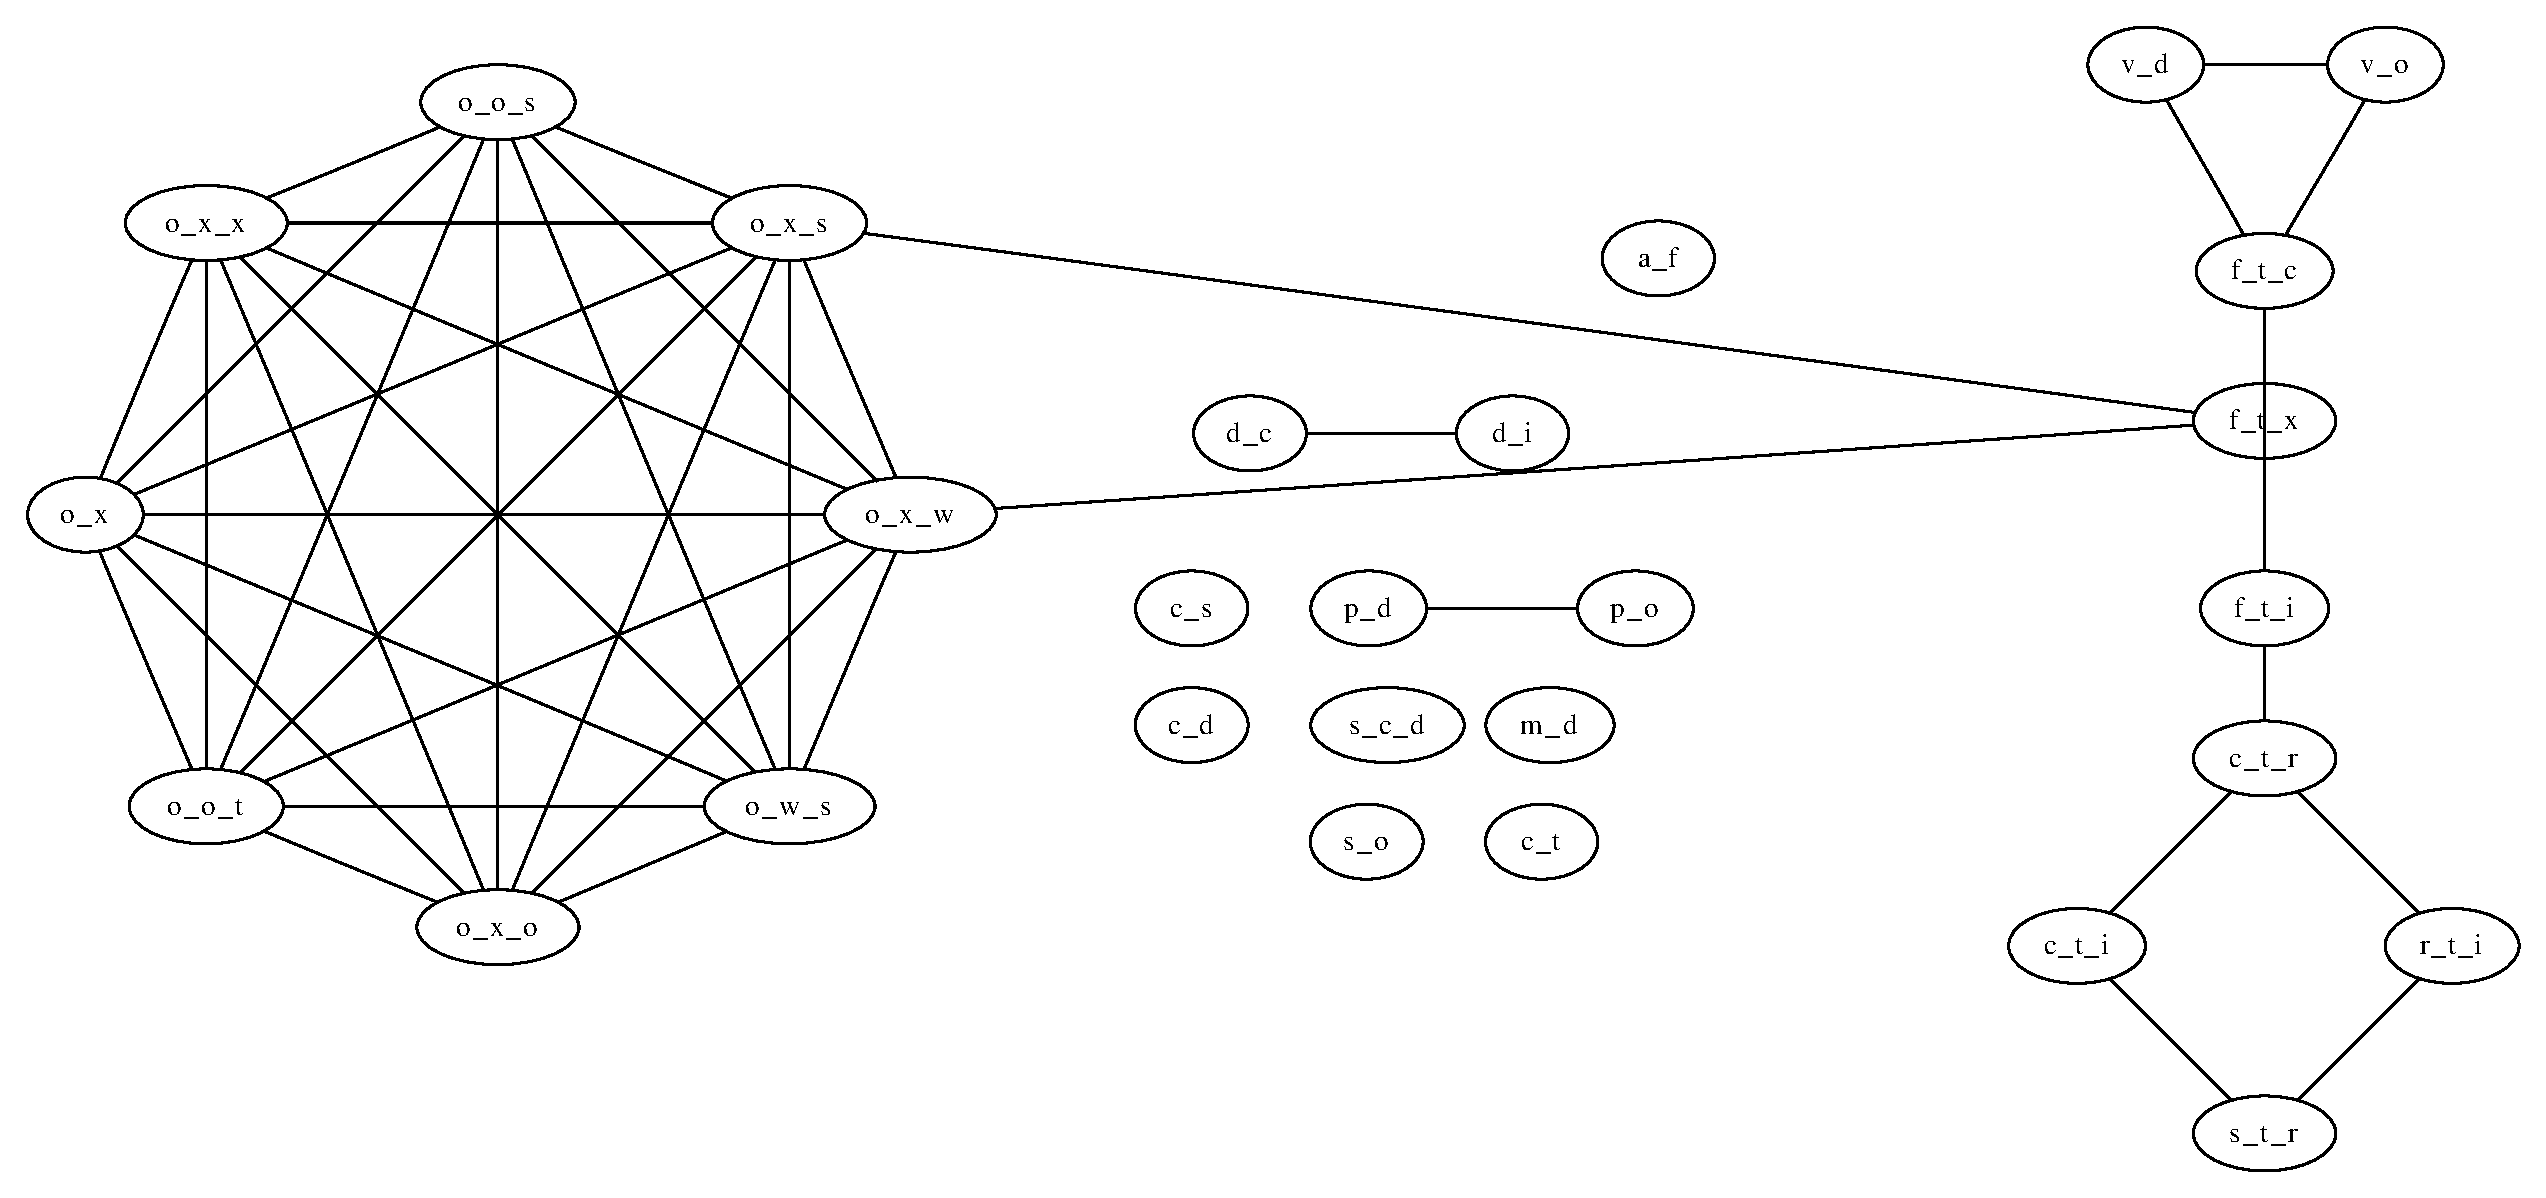
\includegraphics[width=0.45\textwidth]{images/experiments/data/realistic/OVA1}}
    \subfigure[OVA2]{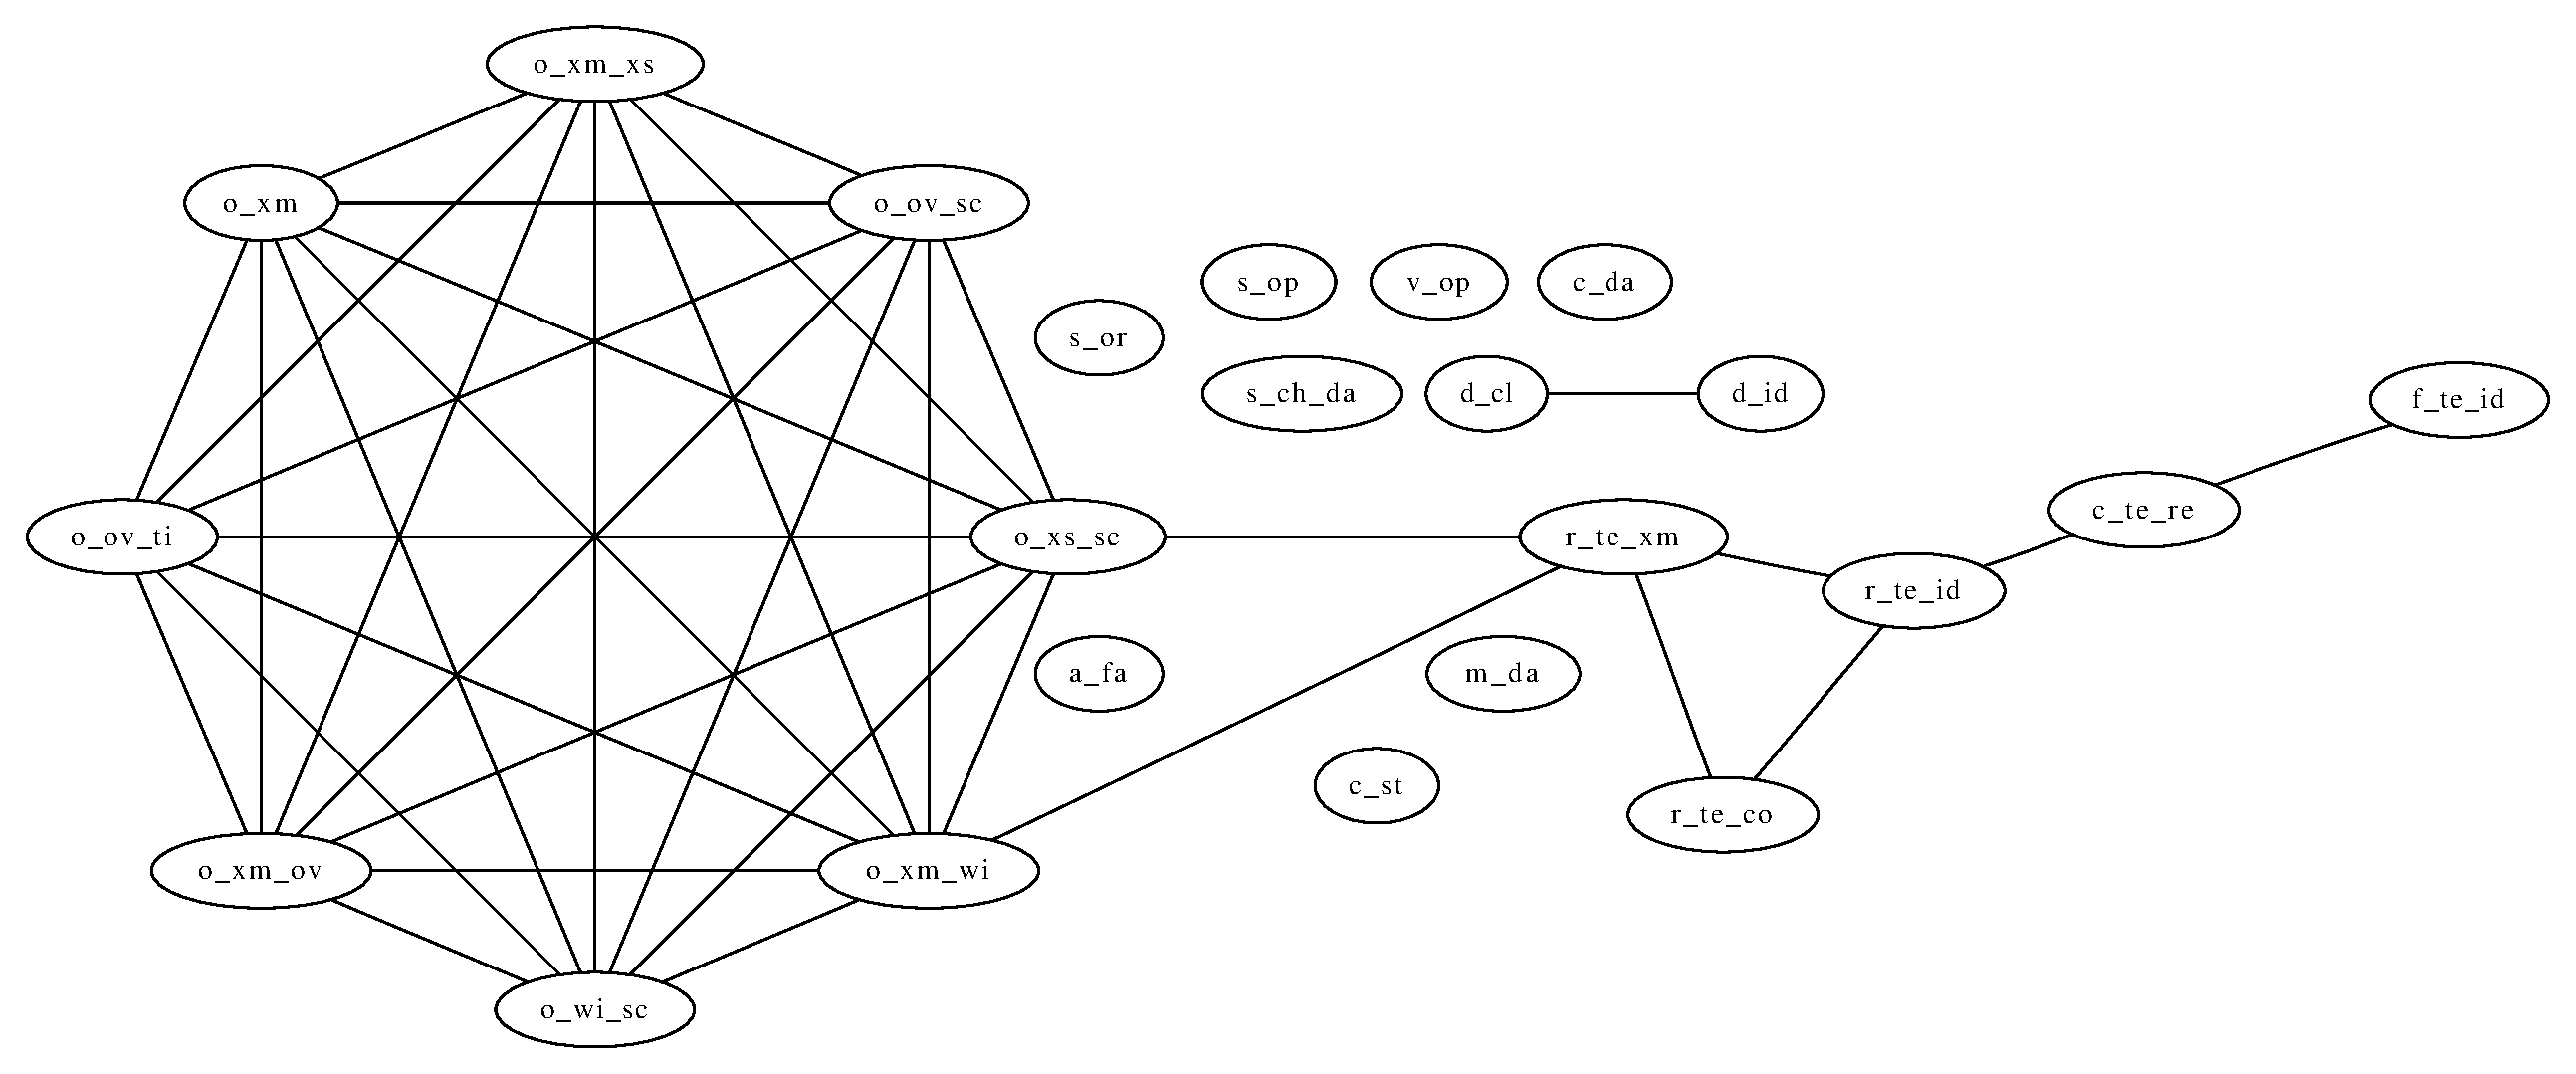
\includegraphics[width=0.45\textwidth]{images/experiments/data/realistic/OVA2}}
    \subfigure[OVA3]{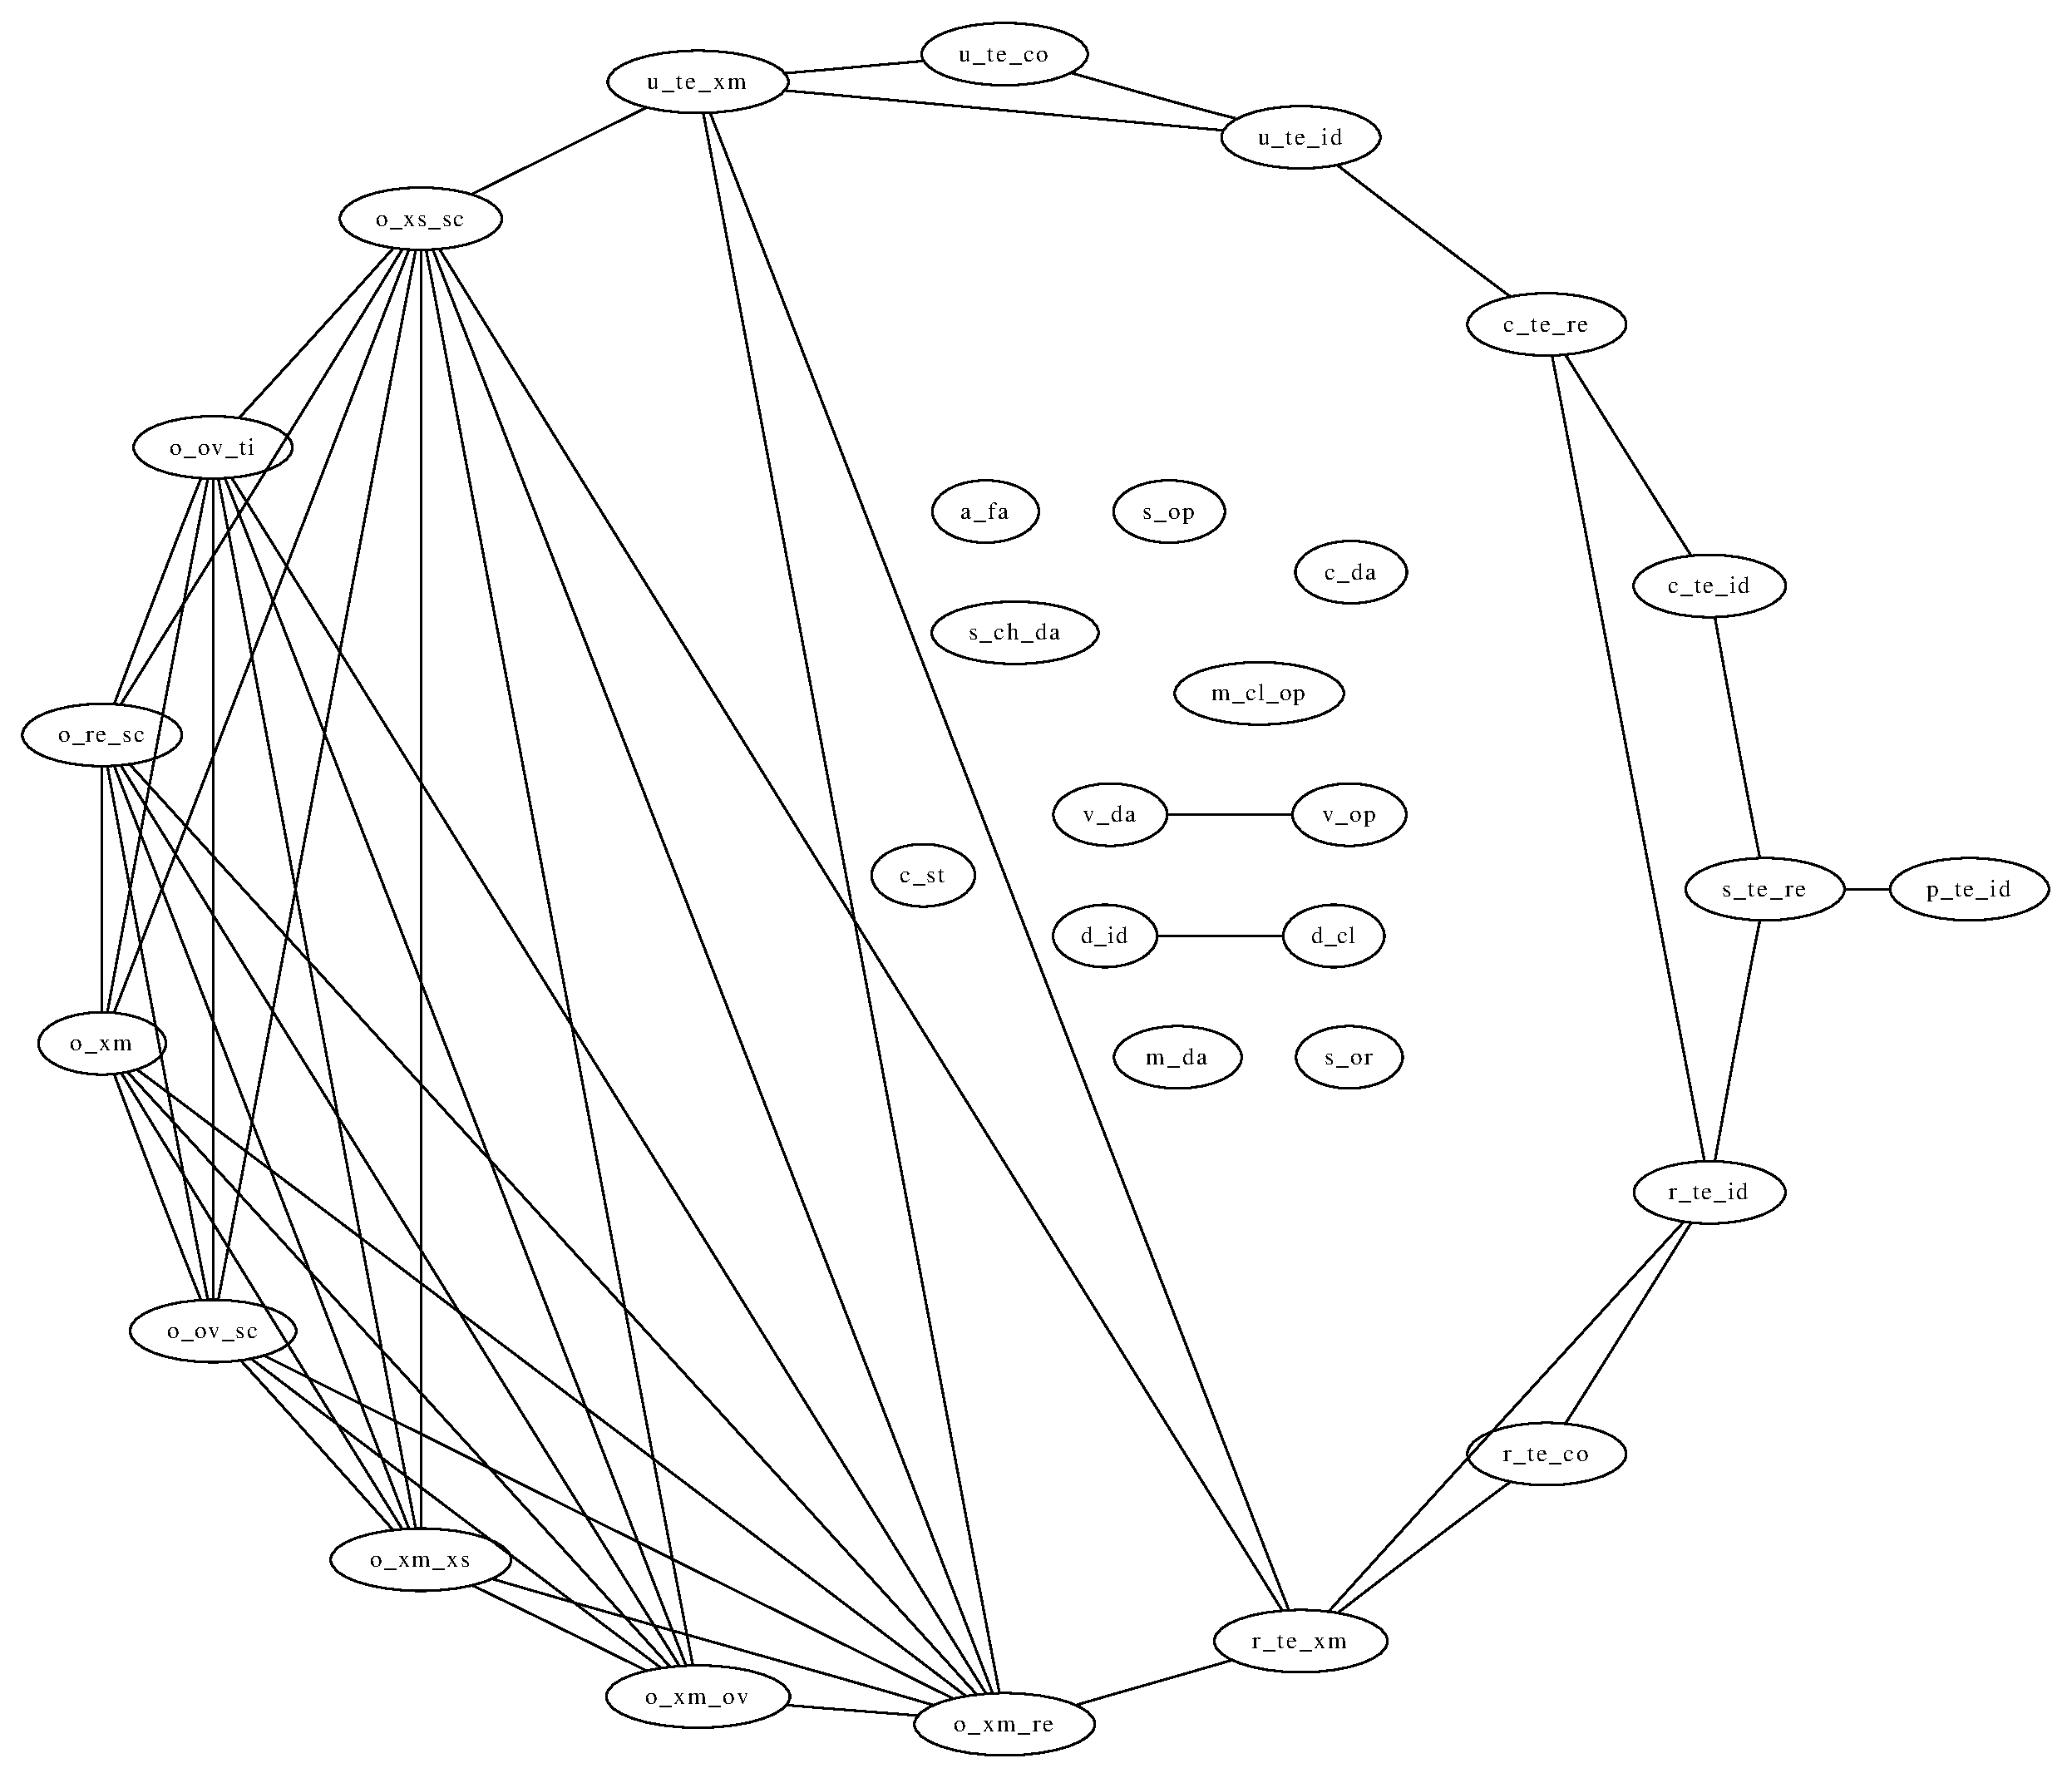
\includegraphics[width=0.45\textwidth]{images/experiments/data/realistic/OVA3}}
    \subfigure[XMA-c]{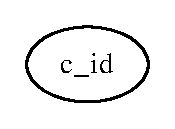
\includegraphics[width=0.08\textwidth]{images/experiments/data/realistic/XMA-c}}
    \subfigure[XMA-p]{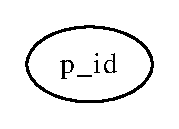
\includegraphics[width=0.08\textwidth]{images/experiments/data/realistic/XMA-p}}
    \subfigure[XMD]{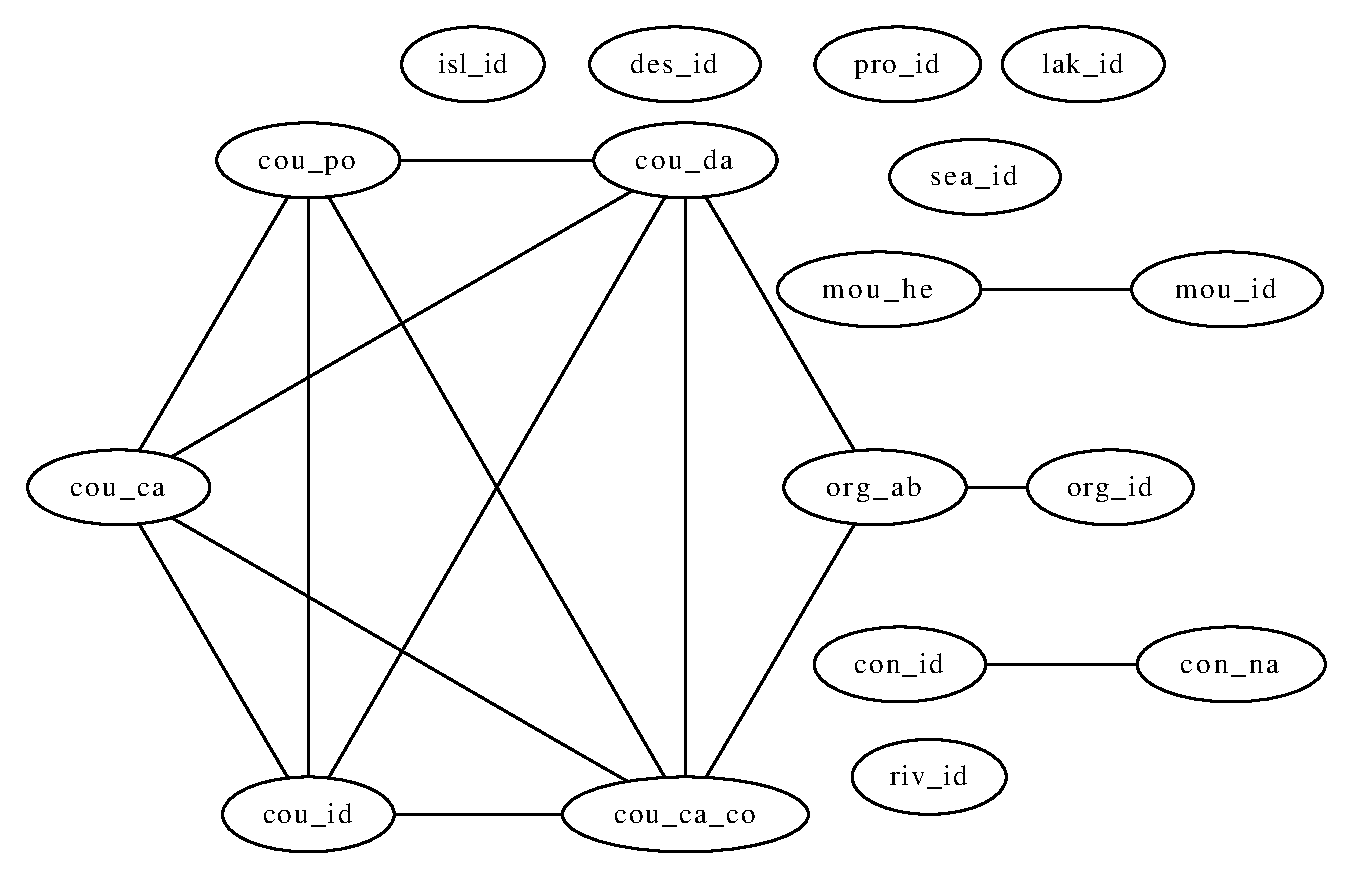
\includegraphics[width=0.45\textwidth]{images/experiments/data/realistic/XMD}}
\end{figure}

To interpret the data a little: \jmodule{OVA*} sets have quite interesting and perhaps a bit challenging graphs, but are not too big. We can consider them to be the ``typical" representants.

On the other hand, the \jmodule{XMA-*} sets are quite huge, but trivial: their only candidate AM will just get picked and that will be the end of the heuristic. We will see the performance of the other components of the whole system, dealing with huge data that are rather simple in the end.

Finally, the \jmodule{XMD} set is quite big and at the same time has non-trivial graph representation. We should see a performance more balanced between processing and finding the ID set here.

\subsection{Realistic data with artificial attributes}
\label{realistic-converted}

We found 2 data sets to convert, \jmodule{MSH} and \jmodule{NTH}. Unfortunately, the same problem with disclosure as in the previous case applies here. None of these sets had any attributes before the conversion. Their summary is the Table \ref{table-experiments-data-converted}, their graphs can be seen in Figure \ref{image-experiments-data-converted}.

TODO schemas?

To address the conversion: in the case of \jmodule{MSH} we found 2 elements with values looking suspiciously like a key of the records contained in the file, and converted them to be attributes of these records using a simple XSL transformation. In the case of \jmodule{NTH} we converted all the values in sub-elements of the record elements to be the attributes of the records.

Why is this useful at all? Recall TODO link, where we said that ID attributes are a special case of XML keys. We can use this approach then to find XML keys: convert some suspicious data into attributes, find the optimal ID set and then create XML key based on this ID set.

\begin{table}
  \caption{List of realistic test data files with converted attributes}
  \bigskip
  \label{table-experiments-data-converted}
  \centering
  \begin{tabular}{l | r | c | c | l}
	Name  & Size [kb] & $|V|$ & $|E|$ & Optimum \\
	\hline
	MSH  & 3 100.5 & 1 & 0 & 0.5416472778036296 \\
	NTH  & 2 523.5 & 5 & 7 & 0.057918595422124436 \\ 
  \end{tabular}
\end{table}

\begin{figure}
  \caption{Realistic data with converted attributes}
  \label{image-experiments-data-converted}
  \centering
    \subfigure[MSH]{
\includegraphics[width=0.08\textwidth]{images/experiments/data/converted/MSH}}
    \subfigure[NTH]{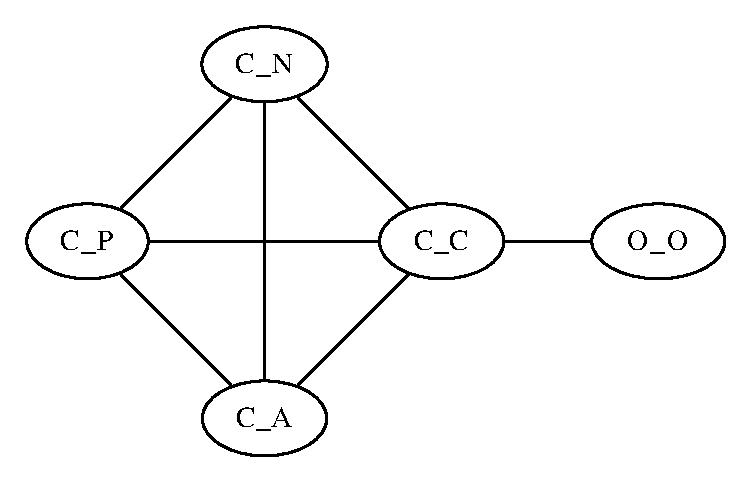
\includegraphics[width=0.45\textwidth]{images/experiments/data/converted/NTH}}
\end{figure}

Again to do a little interpretation: in the case of \jmodule{MSH} we created 2 attributes, of which only one constituted a candidate AM. This is then the case similar to \jmodule{XMA-*} sets: quite large data, yet only one trivial ID attribute to be found.

In the case of \jmodule{NTH} we introduced more attributes, 8 to be precise. Out of them 5 proved to be candidate AMs, with 7 edges constraining them. This means we have quite a big set with relatively simple work to be done by the heuristics. This is about the change.

\subsection{Artificial data}

As soon as we started experimenting with the data coming from the real world, it was obvious that they present no real challenge to our heuristics. After we build the model, we get the most complex graphs of some 31 vertices and 47 edges (see Table \ref{table-experiments-data-realistic}). We needed to create data that would really put pressure on our heuristics, put them to a real test. Our solutions is to approach from the other side: in the end, we will be solving the equivalent of IS problem on a graph created from XML data. Why not create the XML data to contain a more complex graph in the first place? What if we could specify how many vertices and edges we want, and get the according XML?

This is actually simple. Consider the following excerpt from an XML file:

\begin{scriptsize}
\begin{verbatim}
<graph>
  <vertex0 attr="-2968876296119015800"/>
  <vertex1 attr="1729745997570096518"/>
  <vertex2 attr="-9020549659620928934"/>
  ...
  <vertex99 attr="-7545982394508643394"/>

  <vertex82 attr="0"/><vertex21 attr="0"/>
  <vertex64 attr="1"/><vertex21 attr="1"/>
  <vertex44 attr="2"/><vertex2 attr="2"/>
  ...
  <vertex96 attr="99"/><vertex40 attr="99"/>
</graph>
\end{verbatim}
\end{scriptsize}

We want to create a graph with around $v$ vertices and $e$ edges. First, we introduce $v$ elements with names \texttt{vertex0} - \texttt{vertex\{V-1\}}. To constitute an AM, they need an attribute \texttt{attr}, but with large enough random values, so that these values won't conflict with any others. Second, for each of the $e$ edges we pick two \texttt{vertex*} elements at random, and give them the same value of their \texttt{attr}. This will ensure they cannot share the same ID set, thus effectively creating the edge in the graph representation.

The pseudocode for this is in listing \ref{listing-random-data}.

\begin{algorithm}
\caption{Random XML data creation}
\label{listing-random-data}
\begin{algorithmic}
\REQUIRE $v$ requested number of vertices
\REQUIRE $e$ requested number of edges
\ENSURE XML file content
\PRINT \texttt{<graph>}
\FOR{$i = 1 \to |V|$}
	\STATE $R \gets RANDOM$
	\PRINT \texttt{<vertex\textit{i} attr="\textit{R}">}
\ENDFOR
\FOR{$i = 1 \to |E|$}
	\STATE $v1 \gets RANDOM(|V|)$
	\STATE $v2 \gets RANDOM(|V|)$
	\PRINT \texttt{<vertex\textit{v1} attr="\textit{i}"> <vertex\textit{v2} attr="\textit{i}">}
\ENDFOR
\PRINT \texttt{</graph>}
\RETURN
\end{algorithmic}
\end{algorithm}

With this process in place we can create as much data as we wish with any combination of $v$ and $e$ we want.

There is one interesting characteristic that can describe random graphs like this, and that is the \textit{density}. This can be defined in various ways, we will use two different interpretations for a while. The first is $\frac{|E|}{|V|}$, that is, how many edges are there for one vertex (multiplied by 2 we'd get the average degree of the vertices). The second, perhaps more interesting is $\frac{|E|}{E_{max}}$, where $E_{max} = \frac{|V|.(|V|-1)}{2}$. This is the density as the ratio of edges that are to all edges that could be in a complete graph with $|V|$ vertices.

We have created 3 sets to use in experiments along with the realistic and converted sets, these are called \jmodule{100-100}, \jmodule{100-200} and \jmodule{100-1000}. Note that the name is always in the form $v-e$. 

Also, we will need data of comparably similar characteristics but varying size, to study the effects of size on the run times of experiments. For this reason we created 11 more sets, from \jmodule{0-0} as the trivial one to \jmodule{100-500} as the biggest one. We wanted to keep density the same among these sets, and we picked the $\frac{|E|}{E_{max}}$ density interpretation for this.

TODO this is on the DVD.

The summary is the Table \ref{table-experiments-data-artificial} and Table \ref{table-experiments-data-artificial-size}, these tables contain 2 new columns: values of density in both interpretations we introduced. Some graphs can be seen in Figure \ref{image-experiments-data-artificial}.

While studying the tables you might notice that the actual numbers $|V|$ and $|E|$ do not match to the $v$ and $e$ in the names of the sets. This is because how the random generation algorithm works: it might pick the same edge twice, which will automatically render it unsuitable for the ID set (proof is homework). % TODO too much?:)
Because of the so-called Birthday paradox, % TODO link
this will happen more with higher $e$.

\begin{table}
  \caption{List of artificial test data files}
  \bigskip
  \label{table-experiments-data-artificial}
  \centering
  \begin{tabular}{l | r | c | c | c | c | l}
	Name  & Size [kb] & $|V|$ & $|E|$ & $\frac{|E|}{|V|}$ & $\frac{|E|}{E_{max}}$ & Optimum \\
	\hline
	100-100  & 8.4  & 99 & 95  & 0.95 & 0.02 & 0.836666666666667 \\
	100-200  & 13.0 & 96 & 174 & 1.81 & 0.04 & 0.726000000000000 \\ 
    100-1000 & 49.5 & 93 & 754 & 8.11 & 0.16 & 0.380952380952381 \\ 
  \end{tabular}
\end{table}

\begin{table}
  \caption{List of ``sized" artificial test data files}
  \bigskip
  \label{table-experiments-data-artificial-size}
  \centering
  \begin{tabular}{l | r | c | c | c | c | l}
	Name  & Size [kb] & $|V|$ & $|E|$ & $\frac{|E|}{|V|}$ & $\frac{|E|}{E_{max}}$ & Optimum \\
	\hline
	0-0     & 0.2  & 0  & 0   & -    & -    & 0.0                \\
	10-5    & 0.6  & 10 & 5   & 0.50 & 0.11 & 0.8500000000000002 \\ 
    20-20   & 1.7  & 18 & 13  & 0.72 & 0.08 & 0.7166666666666669 \\
   	30-45   & 3.1  & 29 & 43  & 1.48 & 0.11 & 0.7083333333333334 \\ 
	40-80   & 5.1  & 39 & 72  & 1.85 & 0.10 & 0.6950000000000002 \\
	50-125  & 7.5  & 48 & 111 & 2.31 & 0.10 & 0.6566666666666666 \\
	60-180  & 10.4 & 58 & 157 & 2.71 & 0.09 & 0.6214285714285716 \\
	70-245  & 13.8 & 67 & 205 & 3.06 & 0.09 & 0.5982142857142856 \\
	80-320  & 17.6 & 76 & 261 & 3.43 & 0.09 & 0.5791666666666667 \\
	90-405  & 21.9 & 86 & 352 & 4.09 & 0.10 & 0.528888888888889  \\
	100-500 & 26.7 & 91 & 388 & 4.26 & 0.09 & 0.4981818181818182 \\
  \end{tabular}
\end{table}

\begin{figure}
  \caption{Artificial data}
  \label{image-experiments-data-artificial}
  \centering
  	\subfigure[48-80]{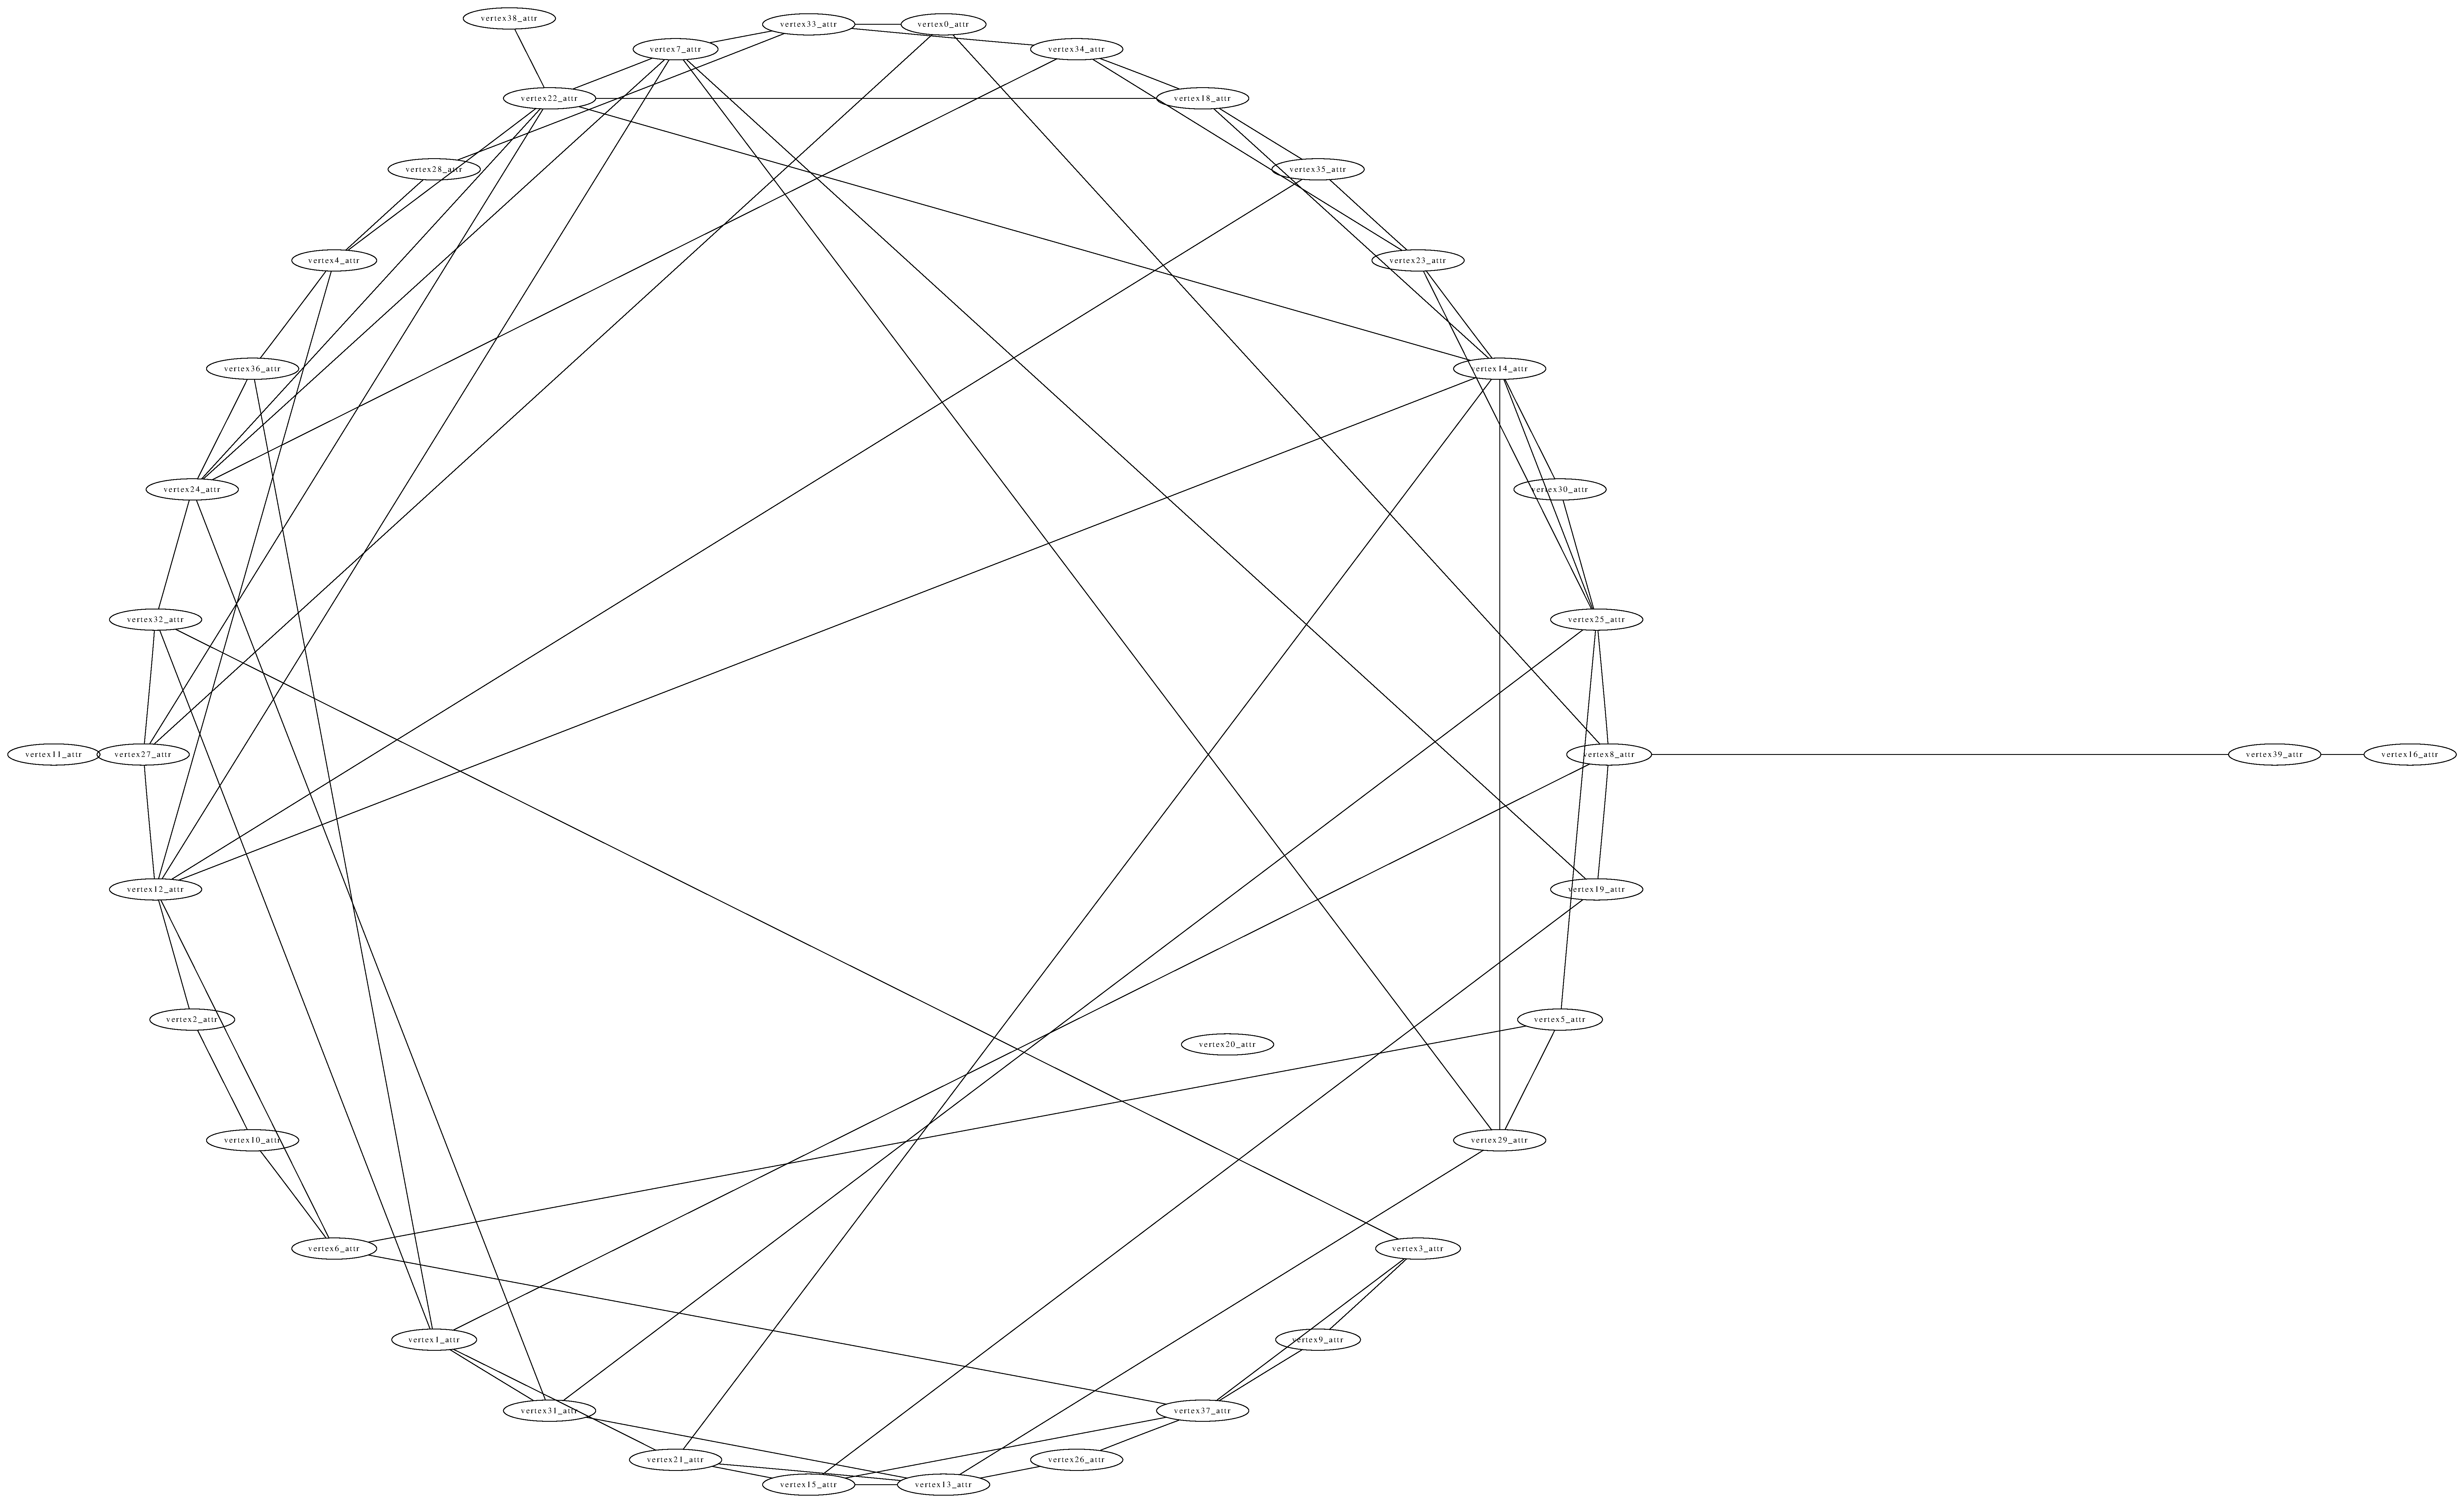
\includegraphics[width=0.45\textwidth]{images/experiments/data/artificial/size/40-80}}
	\subfigure[70-245]{
\includegraphics[width=0.45\textwidth]{images/experiments/data/artificial/size/70-245-fixed}}
\end{figure}

To interpret Tables \ref{table-experiments-data-artificial} and \ref{table-experiments-data-artificial-size}: we get 3 sets of different sizes and densities in the first one, which should work very nice with our heuristics. The $|V|$ and $|E|$ numbers are orders of magnitude higher than with any realistic (or converted) data set we are using, and this will put real stress on the heuristics, as we shall see in the next section.

In the second table we aimed for the $\frac{|E|}{E_{max}}$ density of $0.1 = 10\%$, and we can see that this was quite nicely achieved. There is an interesting observation to be made here: the optimum is steadily decreasing with the increasing overall graph size. This intuitively suggests that the maximal quality theoretically achievable has to do with the $\frac{|E|}{|V|}$ density, not with the one we fixed. Exploration of this phenomenon is among the possibilities of future work of this thesis.

\section{Experimental Setup}

As was mentioned before, we will be using an extension to the jInfer framework called \jmodule{IDSetSearch}. Please see appendices \ref{appendix-jInfer} and \ref{appendix-iss} for more detailed information on these two pieces of software.\\

We now have to define a few notions before moving forward to the description of our experiments.

\begin{define}[Experiment parameters]
	\label{define-experiment-params}
	\textit{Experiment parameters} are the following.
	\begin{itemize}
		\item All the parameters in all the heuristics.
		\item The specific way in which the heuristics are chained.
		\item Parameters $\alpha$ and $\beta$ in the weight (quality) measurement.
		\item Initial pool size.
		\item The termination criteria.
		\item The input XML file.
		\item Known optimum for this file and $\alpha$, $\beta$.
	\end{itemize}
\end{define}

\begin{define}[Experiment(al) configuration]
	\label{define-experiment-config}
	An \textit{experiment instance}, or \textit{configuration}, is one specific setting of all (experiment) parameters.
\end{define}

\begin{define}[Experiment(al) set]
	\label{define-experiment-set}
	One or more experiment configurations, regardless whether their parameters differ, constitute an \textit{experimental set}.
\end{define}

\subsection{Grammar and Model Creation}

TODO link BasicIGG to see how we get IG

TODO describe how we get the model

\subsection{Hardware and Software}

We will be using two different machines to run the experiments. Every experimental result will have explicitly stated the machine it was performed on, and we shall make sure to run different experiments that can benefit from side-by-side comparison on the same machine.

\subsubsection{Linux Machine}

\begin{verbatim}
Intel Core 2 Quad processor @ 2.83 GHz
8 GB DDR2 RAM
x86_64 GNU/Linux 2.6.32-33-generic Ubuntu 10.04
Java HotSpot 64-Bit Server VM (build 20.1-b02)
GLPK version 4.38
\end{verbatim}

\subsubsection{Windows Machine}

\begin{verbatim}
Intel Core 2 Duo processor @ 2.33 GHz
4 GB DDR2 RAM
Windows 7 SP1 64bit
Java HotSpot TODO
GLPK version TODO
\end{verbatim}

\subsection{Methodology}

It is impossible to completely shield an experiment from the influence of the environment, but we should try our best. First of all, NetBeans running the experiments is the only relevant program running in the system at that time, as far as this is possible. Unfortunately, the NetBeans itself is quite a large environment with a life on its own, and we would most certainly get more reliable results, if we could run our experiments outside it. This improvement is left for the future work.

Also, every experimental configuration is run 20 times in hope that the effects of any events adversely affecting our results (e.g. OS deciding to run some house cleaning) will be averaged out. Whenever possible, we will always be using boxplots instead of a simple average (or average and variance) to present results of these multiple runs. % TODO discuss caches and the order in which we run the experiments in one set?

\subsection{Measuring the time}

TODO

\subsection{Obtaining the results}

Every run of an experiment produces a trace such as the one presented and commented on in Appendix \ref{appendix-trace}. We can get all the information relevant to that experiment run from this trace alone. An experimental set will produce a number of these traces and store them in plain text files in a folder. Parsing these files to aggregate and collate them might be a tedious task even using tools like \texttt{sed} and \texttt{grep}, so some of the experiment sets directly output tabular data in format recognized by GnuPlot, which we use to plot charts found in this work.

\section{Experimental Results}

\subsection{GLPK: native vs. Cygwin}

In this experiment we will try to remove one of the variables out of the equation: that is the effect of different versions of GLPK on the overall results. The rationale is this: on Windows systems, the two most accessible ways to install GLPK are via a binary distribution TODO link, or via Cygwin as one of its packages.

If we find out which of these Cygwin version is better, we will be using it exclusively without very much fear that this could affect any other aspect of our experiments. We might also find that there is no relevant difference, which would be good, too.

\begin{table}
  \caption{GLPK: native vs. Cygwin summary}
  \label{experiment-glpk-native-vs-cygwin-summary}
  \centering
  \begin{tabular}{| l | l |}
  \hline
  Machine           & Windows \\
  Input data set    & \texttt{100-500} \\
  Iterations        & 20 \\
  Pool size         & 1 \\
  $\alpha$, $\beta$ & $1$, $1$ \\
  \hline
  \end{tabular}
\end{table}

Our experimental set will contain 500 experimental configurations for each of these two GLPK version. Every configuration will use \jmodule{Glpk} CH set to a time limit from 1 to 49 seconds with increments of 2, meaning 25 settings * 20 iterations = 500 configurations in total (pseudocode to be found in \ref{listing-experiment-glpk-native-vs-cygwin}). There will be no improvement heuristic. The only data we gather in the GnuPlot file are the final qualities (weights).

\begin{algorithm}
\caption{GLPK: native vs. Cygwin generation}
\label{listing-experiment-glpk-native-vs-cygwin}
\begin{algorithmic}
\ENSURE experimental set $ES$
\STATE $ES \gets \emptyset$
\FOR{$i = 1 \to 20$}
	\FOR{$time = 1 \to 49 step 2$}
    \STATE $ES \gets IH = $ \jmodule{Glpk} $, limit = time, IH = \emptyset$  
  \ENDFOR
\ENDFOR
\RETURN $ES$
\end{algorithmic}
\end{algorithm}

TODO input -> time dependency too

\subsection{Still to do}

TODO following experiments + more

\begin{itemize}
	\item For each input file: how long does model creation take?
	\item How long does it take to communicate with GLPK? Creating the input / parsing the output.
	\item Which construction heuristic is the best - limit GLPK to like 1 second
	\item With the best construction heuristic, which IH is the best? Note that this needn't be the best combination!
	\item With the best IH from the previous step, how about using Random as CH?
	\item GLPK: Input -> How long the search for optimum lasts - this shows we cannot rely on GLPK alone! it just takes too long.
	\item GLPK: Time limit -> Quality
	\item Structure of the data -> Which algorithms perform the best
	\item Alpha, Beta -> Quality
	\item Alpha, Beta -> How does the solution work?
	\item Do I beat FIDAX with Random?
	\item Does Fuzzy beat Random? (Fuzzy wins in every single case) - take note of quality (mean, variance) but also time (again, mean)
  \item Can FIDAX be improved by Hungry?
  \item Can we improve performance on huge data by ignoring textual content? Check for building as well as actual heu times.
\end{itemize}

\section{The "Best" Algorithm}

TODO we have asked a lot of questions and got the answers, now is the time to summarize, to find some "wisdom".

First of all: if we have the time, it is best to just let the GLPK run. 
We will find the optimum in this way. 
And for many purposes, this is just fine - we need to infer something about the schema, we do it only once, so it doesn't matter that much how long it takes.

Second: if we don't have enough time, we should do XYZ but it might depend on the characteristics of the data.
For realistic (looks like THIS in graph representation) it is best to do A B C.
Whereas, for artificial data (having IJK as their representation) it is best to just do 1 2 3.

\chapter{Future work}

TODO 

\begin{itemize}
  \item extension to more documents at once
  \item more heuristics and their chaining
  \item ACO, genetic, ...
  \item user-friendly experimental interface (choose and setup experiments on the fly in GUI)
  \item jInfer is opensource, thus easy to extend!
\end{itemize}

\chapwithtoc{Conclusion}

TODO conclusion: From all integrity constraints in XML we chose the ID attributes and decided to improve the search for them. We discussed the approach chosen in FIDAX. Based on this article we introduced the MIP approach and demonstrated how to find the optimal (w.r.t. weight) ID set.

However, this approach takes too long for some inputs, so we introduced a whole spectrum of construction as well as improvement heuristics. By combining these algorithms and tuning their parameters we were able to find very good solutions while maintaining low running times.

%%% Seznam použité literatury
\newpage
\nocite{*}
\bibliographystyle{alpha}
\bibliography{literature}

\listoffigures
\addcontentsline{toc}{chapter}{List of Figures}

\listofalgorithms
\addcontentsline{toc}{chapter}{List of Algorithms}

%%% Tabulky v diplomové práci, existují-li.
%\chapwithtoc{List of Tables}
\listoftables
\addcontentsline{toc}{chapter}{List of Tables}

%%% Použité zkratky v diplomové práci, existují-li, včetně jejich vysvětlení.

\printnomenclature[2cm]
\addcontentsline{toc}{chapter}{List of Abbreviations}

%%% Přílohy k diplomové práci, existují-li (různé dodatky jako výpisy programů,
%%% diagramy apod.). Každá příloha musí být alespoň jednou odkazována z vlastního
%%% textu práce. Přílohy se číslují.

\appendix

\openright
\addcontentsline{toc}{chapter}{Appendices}

\chapter{jInfer}
\label{appendix-jInfer}

This appendix will try to describe shortly yet comprehensively \textbf{jInfer} - the Java framework for XML schema inference. Please see TODO link jInfer project web for complete information, documentation and download options.

jInfer was developed between 2009 and 2011 at Charles University in Prague as a Software Project by team consisting of Michal Klempa, Mario Mikula, Ro\-bert Sme\-ta\-na, Michal Svirec and Matej Vitasek. The main idea was to create a structure in which all aspects of XML schema inference can be easily implemented and evaluated. The goal was apparently achieved: the SW project was successfuly defended when jInfer was inferring DTD and XSD schemas based on XML documents, old DTD and XSD schemas and XPath queries. Since then, Michal Klempa has successfuly defended his own thesis improving on the grammar simplification process (see below), Michal Svirec has extended the framework with capabilities to detect and repair functional dependencies violation and defended his thesis as well. This thesis is the third based on this framework, and Mario Mikula's is on its way, too.

To the best of our knowledge, at the time of writing this thesis is jInfer the only public, open source and actually working solution for XML schema inference-related tasks.

At heart of jInfer inference process is a modular system provided by NetBeans Platform allowing to define services (interfaces), implement them in any number of ways and then let the user choose which implementation to use. Most importantly, the whole process consists of 3 consecutive steps (see \ref{image-inference-process}), responsibility of 3 different services - interchangeable modules.

\begin{figure}
  \caption{Inference process in jInfer}
  \label{image-inference-process}
  \centering
    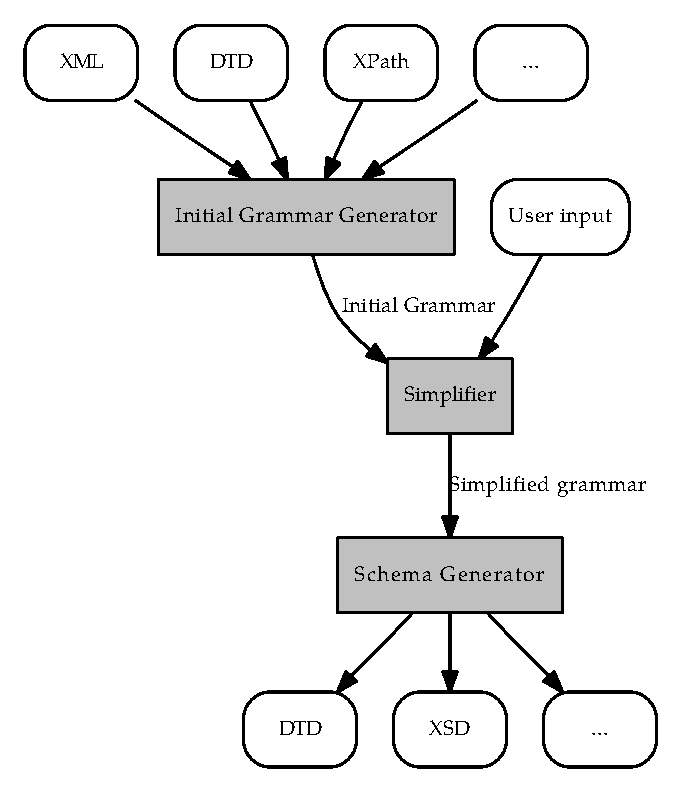
\includegraphics[width=0.5\textwidth]{images/inference-process}
\end{figure}

The responsibility of the first module, the \jmodule{Initial Grammar Generator}, is to parse all input files (documents, schemas and queries) and create a so-called \textit{initial grammar} (IG, TODO nomenclature). This is the representation in which will the structure live until it is used to create the final product - the schema. As the name suggests, IG is a grammar - an \textit{extended context-free grammar}, to be more precise (TODO link CFGs). As such, its left hand side is an element, its right hand side is a regular expression representing its content model. (TODO picture?) IG is used to create the AM model used in this thesis, too. jInfer contains one such module, the \jmodule{BasicIGG}, which is described in detail in (TODO link BasicIGG documentation).

After leaving the \jmodule{Initial Grammar Generator}, the IG needs to be made more general, shortened, \textit{simplified}. This is the responsibility of an aptly named module, the \jmodule{Simplifier}. To get the full idea about how this can be done it would be probably best to read Michal Klempa's thesis (TODO link), which describes this in great detail. Whatever happens, there is simplified grammar on the exit of \jmodule{Simplifier}, ready to be processed by...

The last module, \jmodule{Schema Generator} takes the simplified grammar and creates the resulting schema from it. This process is not too interesting, but anyone wishing to find out all about it is invited to read the documentation to the two \jmodule{Schema Generator}s bundled with jInfer - the BasicDTD and BasicXSD modules.

\chapter{IDSetSearch}
\label{appendix-iss}

TODO talk a bit about the structure of ISS module.

TODO name of the module, its place in jInfer, interface with the framework (service providing)

TODO package name root

TODO "Attribute Stats"

TODO heuristics - interfaces, construction, improvement

TODO experiments - quality, termination, parameters, experiment sets

TODO make sure there was a place where we described the model data model:)

\chapter{Experimental Trace}
\label{appendix-trace}

Following is a trace logged from a sample experiment run. It shows all the relevant information related to this instance, any and every piece of information we might be interested in.

To save space, 2-column layout is used. Commentary on the particulars follows right after its end.

\begin{multicols}{2}
\begin{scriptsize}
\begin{verbatim}
CPU info
  Intel(R) Core(TM)2 Quad CPU Q9550 @ 2.83GHz
  Cores: 4
  Clock speed: 2983 MHz
Memory info
  Size: 8192 MB
OS info
  Name: Windows 7
  Version: 6.1
  Architecture: amd64
Java info
  Version: 1.6.0_26
  VM: Java HotSpot(TM) 64-Bit Server VM
GLPK info
  GLPSOL: GLPK LP/MIP Solver 4.34

Configuration:
File name: graph.xml (101599 b)
  Graph representation: 82 vertices, 1101 edges
alpha: 1.0, beta: 1.0

Results:
Total time spent: 7754 ms
Final quality: 0.19951219512195123 (10 AMs)
Highest quality: 0.23463414634146343 (12 AMs)
Construction phase: 
  Algorithm: Random
    Time taken: 248 ms
    Time since start: 248 ms
    Pool size: 10
    Quality: 0.19975609756097568 (11 AMs)
Improvement phase: 
  pass #1: 
  Algorithm: RandomRemove, ratio = 0.2
    Time taken: 0 ms
    Time since start: 841 ms
    Pool size: 10
    Quality: 0.15878048780487808 (9 AMs)
  pass #2: 
  Algorithm: Mutation, ratio = 0.1, limit = 1 s
    Time taken: 1512 ms
    Time since start: 2710 ms
    Pool size: 11
    Quality: 0.21975609756097558 (11 AMs)

  <... 7 more passes removed ...>

  pass #10: 
  Algorithm: Remove Worst
    Time taken: 80 ms
    Time since start: 7676 ms
    Pool size: 12
    Quality: 0.19951219512195123 (10 AMs)
Termination reason: Max\-imum ite\-rat\-ions ex\-cee\-ded.

Time,Quality,AMs
248,0.19975609756097568,11
841,0.15878048780487808,9
2710,0.21975609756097558,11
2927,0.1890243902439024,9
4421,0.23463414634146343,12
4703,0.23463414634146343,12
4896,0.1960975609756098,10
5793,0.23463414634146337,12
5972,0.19951219512195123,10
7433,0.19951219512195123,10
7676,0.19951219512195123,10

ID
Element,Attribute,Weight
vertex0,attr,0.024146341463414635
vertex2,attr,0.01975609756097561
vertex33,attr,0.016829268292682928
vertex34,attr,0.02219512195121951
vertex4,attr,0.022682926829268292
vertex41,attr,0.014878048780487804
vertex7,attr,0.02170731707317073
vertex70,attr,0.018780487804878048
vertex76,attr,0.01780487804878049
vertex8,attr,0.02170731707317073
vertex80,attr,0.01780487804878049
vertex97,attr,0.016341463414634147

IDREF
Element,Attribute
\end{verbatim}
\end{scriptsize}
\end{multicols}

The first section deals with system information. Please note that some of these characteristics cannot be easily obtained programmatically and are thus stored in the source code as constants.\\
To obtain GLPK information, the program parses the first line of standard output produced by running \code{glpsol -v}. It tries to guess whether it's the Cygwin version by looking at the path to the binary.

% TODO make sure G.R. was introduced before! and LINK IT! swedish style!
The second section states the input file along with its size and graph representation.\\
Alpha and beta parameters for this instance belong here too.

\begin{footnotesize}
\begin{verbatim}
Configuration:
File name: graph.xml (101599 b)
  Graph representation: 82 vertices, 1101 edges
alpha: 1.0, beta: 1.0
\end{verbatim}
\end{footnotesize}

Results section opens stating the most important information first: how long did the experiment run and what was the highest and final quality (these two are potentially different). Numbers of attribute mappings in the best and final solution respectively are stated as well.

\begin{footnotesize}
\begin{verbatim}
Total time spent: 7754 ms
Final quality: 0.19951219512195123 (10 AMs)
Highest quality: 0.23463414634146343 (12 AMs)
\end{verbatim}
\end{footnotesize}

Construction phase results go next. Among reported information are the full identification of the heuristic (possibly along with its parameters), time taken, size of the pool created and the quality of the incumbent solution (again, with the number of its AMs).

\begin{footnotesize}
\begin{verbatim}
Algorithm: Random
  Time taken: 248 ms
  Time since start: 248 ms
  Pool size: 10
  Quality: 0.19975609756097568 (11 AMs)
\end{verbatim}
\end{footnotesize}

Now for each of the improvement phases there is one section in output log. Information presented here has the same structure as with the construction phase. Please note that the \code{Pool size} is always measured \textit{after} the improvement run.

\begin{footnotesize}
\begin{verbatim}
Algorithm: Mutation, ratio = 0.1, limit = 1 s
  Time taken: 1512 ms
  Time since start: 2710 ms
  Pool size: 11
  Quality: 0.21975609756097558 (11 AMs)
\end{verbatim}
\end{footnotesize}

After the last improvement phase, the reason why the metaheuristic terminated is stated. Possible causes are exceeding the maximum time available, maximum iterations or reaching the known optimum for this file and alpha / beta settings.
\\

To be able to reconstruct the progress of the metaheuristic, the next section contains CSV \nomenclature{CSV}{Comma Separated Values} formatted data for each iteration. Each row contains the time in milliseconds, quality of the incumbent solution and the number of its AMs.

\begin{footnotesize}
\begin{verbatim}
Time,Quality,AMs
...
841,0.15878048780487808,9
2710,0.21975609756097558,11
...
\end{verbatim}
\end{footnotesize}

And finally, it is important to know what is the ID/IDREF set recommended by this experiment run - the reason why we do all this! Thus the log is concluded by a CSV formatted list of element - attribute name pairs to be included in the ID and IDREF set, respectively.

\begin{footnotesize}
\begin{verbatim}
Element,Attribute,Weight
vertex0,attr,0.024146341463414635
...
\end{verbatim}
\end{footnotesize}

Note that in this example trace there were no IDREF AMs found.

\flushright
$\square$

\end{document}
